\begin{frame}[fragile]{Tutorial: Two-site circuit optimization}

\begin{columns}

\begin{column}{5cm}

\begin{onlyenv}<1->
\begin{lstlisting}[language=JuliaLocal, style=julia, mathescape, basicstyle=\scriptsize\ttfamily]
$\psi$0 = Zp1 * Zp2


function E($\theta$)
  $\psi\theta$ = apply(U($\theta$,i1,i2),$\psi$0)
  return inner($\psi\theta$',H,$\psi\theta$)
end
\end{lstlisting}
\end{onlyenv}

\begin{onlyenv}<3->
\begin{lstlisting}[language=JuliaLocal, style=julia, mathescape, basicstyle=\scriptsize\ttfamily]
$\theta$0 = [0, 0, 0, 0]
$\partial$E($\theta$) = gradient(E, $\theta$)[1]
$\theta$ = minimize(E, $\partial$E, $\theta$0;
           nsteps=40, $\gamma$=0.5)

E($\theta$0) == -1
E($\theta$) # $\approx$ -1.4142077 $\approx$ -√2
\end{lstlisting}
\end{onlyenv}

\end{column}

\begin{column}{5cm}

\begin{onlyenv}<1-1>
References state: \\
|0$\rangle$ = |Z+Z+$\rangle$ \\
~\\
$\min_{\theta}$ E($\theta$)\\
\ \ = $\min_{\theta}$ $\langle$0|U($\theta$)$^\dagger$ H U($\theta$)|0$\rangle$ \\
\ \ = $\min_{\theta}$ $\langle\theta$|H|$\theta\rangle$ \\
\end{onlyenv}

\begin{onlyenv}<2->
\vspace*{0.0cm}
\begin{center}
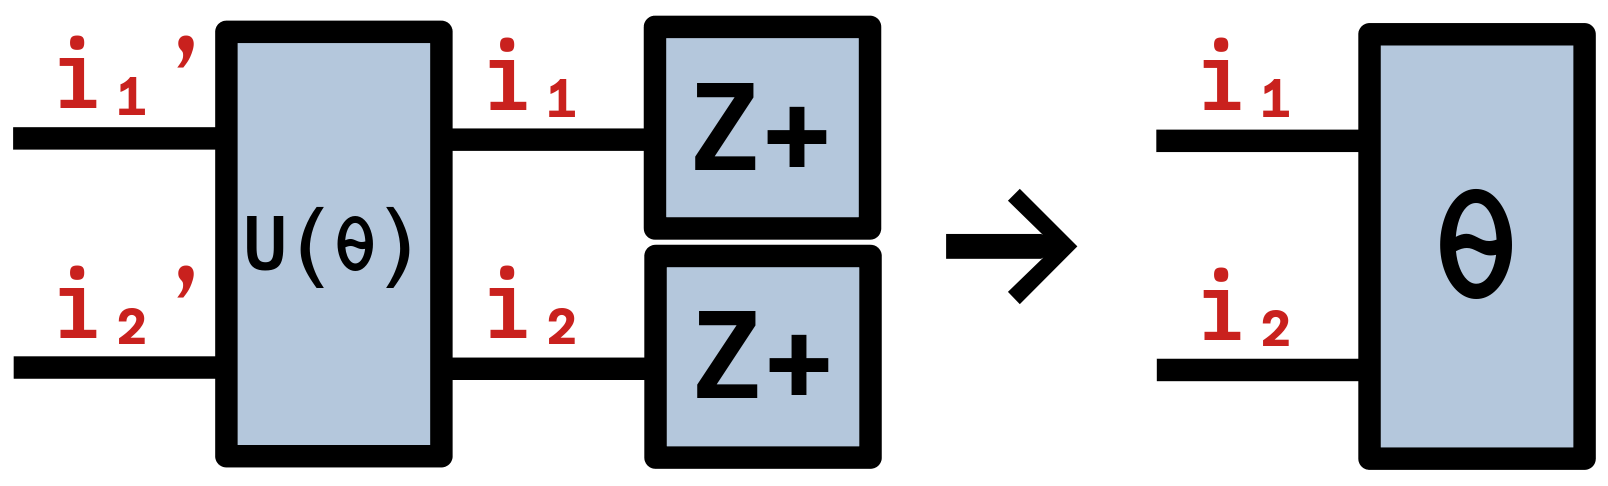
\includegraphics[width=1.0\textwidth]{
  slides/assets/UZp1Zp2.png
} \\
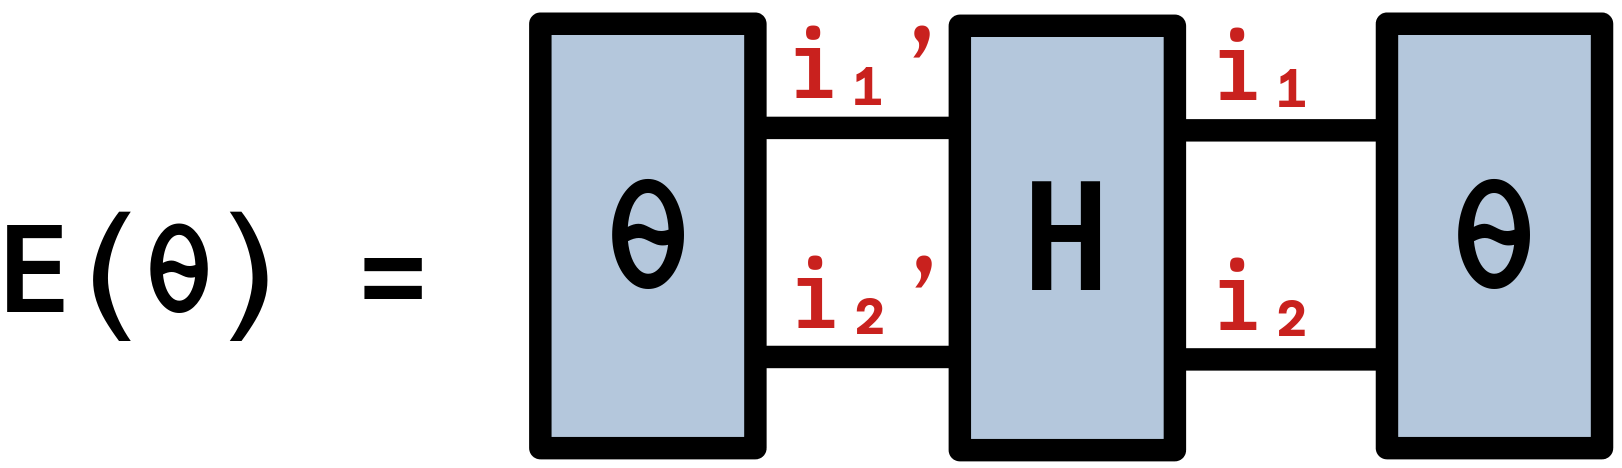
\includegraphics[width=1.0\textwidth]{
  slides/assets/theta12Htheta12.png
}
\end{center}
\vspace*{0.0cm}
\end{onlyenv}

\begin{onlyenv}<3->
\vspace*{0.0cm}
\begin{center}
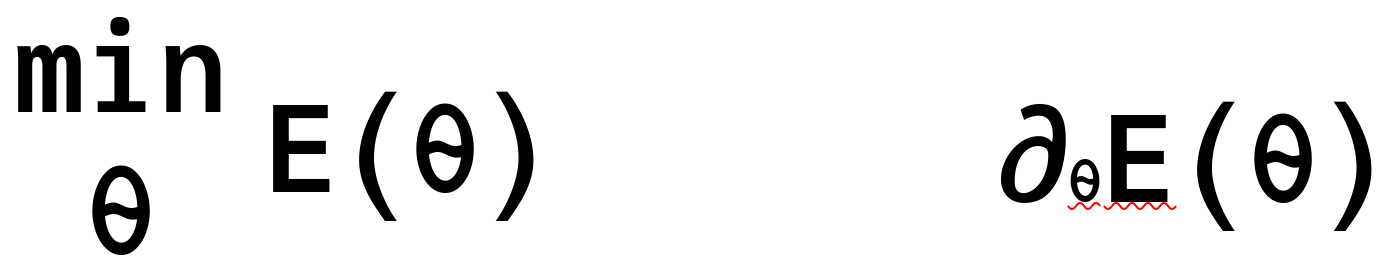
\includegraphics[width=1.0\textwidth]{
  slides/assets/min_grad_E_theta.png
}
\end{center}
%% (-1, √3/2) \\
%% (-1.4142077, 0.0017584116) \\
%%        $\approx$ (-√2, 0) \\
\vspace*{0.0cm}
\end{onlyenv}

\end{column}

\end{columns}

\end{frame}
